%%%%%%%%%%%%%%%%%%%%%%%%%%%%%%%%%%%%%%%%%%%%%%%%%%%%%%%%%%%%%%%%%%%%%%%%%%%%%%%%
%%%%%%%%%%%%%%%%%%%%%%%%%%%%%%%%%%%%%%%%%%%%%%%%%%%%%%%%%%%%%%%%%%%%%%%%%%%%%%%%
%%                                                                            %%
%% thesistemplate.tex version 3.20 (2018/08/31)                               %%
%% The LaTeX template file to be used with the aaltothesis.sty (version 3.20) %%
%% style file.                                                                %%
%% This package requires pdfx.sty v. 1.5.84 (2017/05/18) or newer.            %%
%%                                                                            %%
%% This is licensed under the terms of the MIT license below.                 %%
%%                                                                            %%
%% Written by Luis R.J. Costa.                                                %%
%% Currently developed at the Learning Services of Aalto University School of %%
%% Electrical Engineering by Luis R.J. Costa since May 2017.                  %%
%%                                                                            %%
%% Copyright 2017-2018, by Luis R.J. Costa, luis.costa@aalto.fi,              %%
%% Copyright 2017-2018 Swedish translations in aaltothesis.cls by Elisabeth   %%
%% Nyberg, elisabeth.nyberg@aalto.fi and Henrik Wallén,                       %%
%% henrik.wallen@aalto.fi.                                                    %%
%% Copyright 2017-2018 Finnish documentation in the template opinnatepohja.tex%%
%% by Perttu Puska, perttu.puska@aalto.fi, and Luis R.J. Costa.               %%
%% Copyright 2018 English template thesistemplate.tex by Luis R.J. Costa.     %%
%% Copyright 2018 Swedish template kandidatarbetsbotten.tex by Henrik Wallen. %%
%%                                                                            %%
%% Permission is hereby granted, free of charge, to any person obtaining a    %%
%% copy of this software and associated documentation files (the "Software"), %%
%% to deal in the Software without restriction, including without limitation  %%
%% the rights to use, copy, modify, merge, publish, distribute, sublicense,   %%
%% and/or sell copies of the Software, and to permit persons to whom the      %%
%% Software is furnished to do so, subject to the following conditions:       %%
%% The above copyright notice and this permission notice shall be included in %%
%% all copies or substantial portions of the Software.                        %%
%% THE SOFTWARE IS PROVIDED "AS IS", WITHOUT WARRANTY OF ANY KIND, EXPRESS OR %%
%% IMPLIED, INCLUDING BUT NOT LIMITED TO THE WARRANTIES OF MERCHANTABILITY,   %%
%% FITNESS FOR A PARTICULAR PURPOSE AND NONINFRINGEMENT. IN NO EVENT SHALL    %%
%% THE AUTHORS OR COPYRIGHT HOLDERS BE LIABLE FOR ANY CLAIM, DAMAGES OR OTHER %%
%% LIABILITY, WHETHER IN AN ACTION OF CONTRACT, TORT OR OTHERWISE, ARISING    %%
%% FROM, OUT OF OR IN CONNECTION WITH THE SOFTWARE OR THE USE OR OTHER        %%
%% DEALINGS IN THE SOFTWARE.                                                  %%
%%                                                                            %%
%%                                                                            %%
%%%%%%%%%%%%%%%%%%%%%%%%%%%%%%%%%%%%%%%%%%%%%%%%%%%%%%%%%%%%%%%%%%%%%%%%%%%%%%%%
%%                                                                            %%
%%                                                                            %%
%% An example for writting your thesis using LaTeX                            %%
%% Original version and development work by Luis Costa, changes to the text   %% 
%% in the Finnish template by Perttu Puska.                                   %%
%% Support for Swedish added 15092014                                         %%
%% PDF/A-b support added on 15092017                                          %%
%% PDF/A-2 support added on 24042018                                          %%
%%                                                                            %%
%% This example consists of the files                                         %%
%%         thesistemplate.tex (version 3.20) (for text in English)            %%
%%         opinnaytepohja.tex (version 3.20) (for text in Finnish)            %%
%%         kandidatarbetsbotten.tex (version 1.00) (for text in Swedish)      %%
%%         aaltothesis.cls (versio 3.20)                                      %%
%%         kuva1.eps (graphics file)                                          %%
%%         kuva2.eps (graphics file)                                          %%
%%         kuva1.jpg (graphics file)                                          %%
%%         kuva2.jpg (graphics file)                                          %%
%%         kuva1.png (graphics file)                                          %%
%%         kuva2.png (graphics file)                                          %%
%%         kuva1.pdf (graphics file)                                          %%
%%         kuva2.pdf (graphics file)                                          %%
%%                                                                            %%
%%                                                                            %%
%% Typeset in Linux either with                                               %%
%% pdflatex: (recommended method)                                             %%
%%             $ pdflatex thesistemplate                                      %%
%%             $ pdflatex thesistemplate                                      %%
%%                                                                            %%
%%   The result is the file thesistemplate.pdf that is PDF/A compliant, if    %%
%%   you have chosen the proper \documenclass options (see comments below)    %%
%%   and your included graphics files have no problems.
%%                                                                            %%
%% Or                                                                         %%
%% latex: (this method is not recommended)                                    %%
%%             $ latex thesistemplate                                         %%
%%             $ latex thesistemplate                                         %%
%%                                                                            %%
%%   The result is the file thesistemplate.dvi, which is converted to ps      %%
%%   format as follows:                                                       %%
%%                                                                            %%
%%             $ dvips thesistemplate -o                                      %%
%%                                                                            %%
%%   and then to pdf as follows:                                              %%
%%                                                                            %%
%%             $ ps2pdf thesistemplate.ps                                     %%
%%                                                                            %%
%%   This pdf file is not PDF/A compliant. You must must make it so using,    %%
%%   e.g., Acrobat Pro or PDF-XChange.                                        %%
%%                                                                            %%
%%                                                                            %%
%% Explanatory comments in this example begin with the characters %%, and     %%
%% changes that the user can make with the character %                        %%
%%                                                                            %%
%%%%%%%%%%%%%%%%%%%%%%%%%%%%%%%%%%%%%%%%%%%%%%%%%%%%%%%%%%%%%%%%%%%%%%%%%%%%%%%%
%%%%%%%%%%%%%%%%%%%%%%%%%%%%%%%%%%%%%%%%%%%%%%%%%%%%%%%%%%%%%%%%%%%%%%%%%%%%%%%%
%%
%% WHAT is PDF/A
%%
%% PDF/A is the ISO-standardized version of the pdf. The standard's goal is to
%% ensure that he file is reproducable even after a long time. PDF/A differs
%% from pdf in that it allows only those pdf features that support long-term
%% archiving of a file. For example, PDF/A requires that all used fonts are
%% embedded in the file, whereas a normal pdf can contain only a link to the
%% fonts in the system of the reader of the file. PDF/A also requires, among
%% other things, data on colour definition and the encryption used.
%% Currently three PDF/A standards exist:
%% PDF/A-1: based on PDF 1.4, standard ISO19005-1, published in 2005.
%%          Includes all the requirements essential for long-term archiving.
%% PDF/A-2: based on PDF 1.7, standard ISO19005-2, published in 2011.
%%          In addition to the above, it supports embedding of OpenType fonts,
%%          transparency in the colour definition and digital signatures.
%% PDF/A-3: based on PDF 1.7, standard ISO19005-3, published in 2012.
%%          Differs from the above only in that it allows embedding of files in
%%          any format (e.g., xml, csv, cad, spreadsheet or wordprocessing
%%          formats) into the pdf file.
%% PDF/A-1 files are not necessarily PDF/A-2 -compatible and PDF/A-2 are not
%% necessarily PDF/A-1 -compatible.
%% All of the above PDF/A standards have two levels:
%% b: (basic) requires that the visual appearance of the document is reliably
%%    reproduceable.
%% a (accessible) in addition to the b-level requirements, specifies how
%%   accessible the pdf file is to assistive software, say, for the physically
%%   impaired.
%% For more details on PDF/A, see, e.g., https://en.wikipedia.org/wiki/PDF/A
%%
%%
%% WHICH PDF/A standard should my thesis conform to?
%%
%% Primarily to the PDF/A-1b standard. All the figures and graphs typically
%% use in thesis work do not require transparency features, a basic '2-D'
%% visualisation suffices. The font to be used are specified in this template
%% and they should not be changed. However, if you have figures where
%% transparency characteristics matter, use the PDF/A-2b standard. Do not use
%% the PDF/A-3b standard for your thesis.
%%
%%
%% WHAT graphics format can I use to produce my PDF/A compliant file?
%%
%% When using pdflatex to compile your work, use jpg, png or pdf files. You may
%% have PDF/A compliance problems with figures in pdf format. Do not use PDF/A
%% compliant graphics files.
%% If you decide to use latex to compile your work, the only acceptable file
%% format for your figure is eps. DO NOT use the ps format for your figures.

%% USE one of these:
%% * the first when using pdflatex, which directly typesets your document in the
%%   chosen pdf/a format and you want to publish your thesis online,

%% * the second when you want to print your thesis to bind it, or
%% * the third when producing a ps file and a pdf/a from it.
%%
\documentclass[english, 12pt, a4paper, elec, utf8, a-1b, online]{aaltothesis}
%\documentclass[english, 12pt, a4paper, elec, utf8, a-1b]{aaltothesis}
%\documentclass[english, 12pt, a4paper, elec, dvips, online]{aaltothesis}

%% Use the following options in the \documentclass macro above:
%% your school: arts, biz, chem, elec, eng, sci
%% the character encoding scheme used by your editor: utf8, latin1
%% thesis language: english, finnish, swedish
%% make an archiveable PDF/A-1b or PDF/A-2b compliant file: a-1b, a-2b
%%                    (with pdflatex, a normal pdf containing metadata is
%%                     produced without the a-*b option)
%% typeset in symmetric layout and blue hypertext for online publication: online
%%            (no option is the default, resulting in a wide margin on the
%%             binding side of the page and black hypertext)
%% two-sided printing: twoside (default is one-sided printing)
%%

%% Use one of these if you write in Finnish (see the Finnish template
%% opinnaytepohja.tex)
%\documentclass[finnish, 12pt, a4paper, elec, utf8, a-1b, online]{aaltothesis}
%\documentclass[finnish, 12pt, a4paper, elec, utf8, a-1b]{aaltothesis}
%\documentclass[finnish, 12pt, a4paper, elec, dvips, online]{aaltothesis}

\usepackage{graphicx}

%% Math fonts, symbols, and formatting; these are usually needed
\usepackage{amsfonts,amssymb,amsbsy,amsmath}

%% Change the school field to specify your school if the automatically set name
%% is wrong
% \university{aalto-yliopisto}
% \school{Sähkötekniikan korkeakoulu}

%% Edit to conform to your degree programme
%%
\degreeprogram{Electronics and electrical engineering}
%%

%% Your major
%%
\major{An appropriate major}
%%

%% Major subject code
%%
\code{ELEC0007}
%%
 
%% Choose one of the three below
%%
\univdegree{BSc}
%\univdegree{MSc}
%\univdegree{Lic}
%%

%% Your name (self explanatory...)
%%
\thesisauthor{Eddie Engineer}
%%

%% Your thesis title comes here and possibly again together with the Finnish or
%% Swedish abstract. Do not hyphenate the title, and avoid writing too long a
%% title. Should LaTeX typeset a long title unsatisfactorily, you mght have to
%% force a linebreak using the \\ control characters.
%% In this case...
%% Remember, the title should not be hyphenated!
%% A possible "and" in the title should not be the last word in the line, it
%% begins the next line.
%% Specify the title again without the linebreak characters in the optional
%% argument in box brackets. This is done because the title is part of the 
%% metadata in the pdf/a file, and the metadata cannot contain linebreaks.
%%
\thesistitle{Title of the thesis}
%\thesistitle[Title of the thesis]{Title of\\ the thesis}
%%

%%
\place{Espoo}
%%

%% The date for the bachelor's thesis is the day it is presented
%%
\date{31.8.2018}
%%

%% Thesis supervisor
%% Note the "\" character in the title after the period and before the space
%% and the following character string.
%% This is because the period is not the end of a sentence after which a
%% slightly longer space follows, but what is desired is a regular interword
%% space.
%%
\supervisor{Prof.\ Pirjo Professor}
%%

%% Advisor(s)---two at the most---of the thesis. Check with your supervisor how
%% many official advisors you can have.
%%
\advisor{Dr Alan Advisor}
%\advisor{MSc Sarah Scientist}
%%

%% Aaltologo: syntax:
%% \uselogo{aaltoRed|aaltoBlue|aaltoYellow|aaltoGray|aaltoGrayScale}{?|!|''}
%% The logo language is set to be the same as the thesis language.
%%
\uselogo{aaltoRed}{''}
%%

%% The English abstract:
%% All the details (name, title, etc.) on the abstract page appear as specified
%% above.
%% Thesis keywords:
%% Note! The keywords are separated using the \spc macro
%%
\keywords{For keywords choose\spc concepts that are\spc central to your\spc thesis}
%%

%% The abstract text. This text is included in the metadata of the pdf file as well
%% as the abstract page.
%%
\thesisabstract{
Your abstract in English. Keep the abstract short. The abstract explains your 
research topic, the methods you have used, and the results you obtained. In the 
PDF/A format of this thesis, in addition to the abstract page, the abstract text is 
written into the pdf file's metadata. Write here the text that goes into the 
metadata. The metadata cannot contain special characters, linebreak or paragraph 
break characters, so these must not be used here. If your abstract does not contain 
special characters and it does not require paragraphs, you may take advantage of 
the abstracttext macro (see the comment below). Otherwise, the metadata abstract 
text must be identical to the text on the abstract page.
}

%% Copyright text. Copyright of a work is with the creator/author of the work
%% regardless of whether the copyright mark is explicitly in the work or not.
%% You may, if you wish, publish your work under a Creative Commons license (see
%% creaticecommons.org), in which case the license text must be visible in the
%% work. Write here the copyright text you want. It is written into the metadata
%% of the pdf file as well.
%% Syntax:
%% \copyrigthtext{metadata text}{text visible on the page}
%% 
%% In the macro below, the text written in the metadata must have a \noexpand
%% macro before the \copyright special character, and macros (\copyright and
%% \year here) must be separated by the \ character (space chacter) from the
%% text that follows. The macros in the argument of the \copyrighttext macro
%% automatically insert the year and the author's name. (Note! \ThesisAuthor is
%% an internal macro of the aaltothesis.cls class file).
%% Of course, the same text could have simply been written as
%% \copyrighttext{Copyright \noexpand\copyright\ 2018 Eddie Engineer}
%% {Copyright \copyright{} 2018 Eddie Engineer}
%%
\copyrighttext{Copyright \noexpand\copyright\ \number\year\ \ThesisAuthor}
{Copyright \copyright{} \number\year{} \ThesisAuthor}

%% You can prevent LaTeX from writing into the xmpdata file (it contains all the 
%% metadata to be written into the pdf file) by setting the writexmpdata switch
%% to 'false'. This allows you to write the metadata in the correct format
%% directly into the file thesistemplate.xmpdata.
%\setboolean{writexmpdatafile}{false}

%% All that is printed on paper starts here
%%
\begin{document}

%% Create the coverpage
%%
\makecoverpage

%% Typeset the copyright text.
%% If you wish, you may leave out the copyright text from the human-readable
%% page of the pdf file. This may seem like a attractive idea for the printed
%% document especially if "Copyright (c) yyyy Eddie Engineer" is the only text
%% on the page. However, the recommendation is to print this copyright text.
%%
\makecopyrightpage

%% Note that when writting your thesis in English, place the English abstract
%% first followed by the possible Finnish or Swedish abstract.

%% Abstract text
%% All the details (name, title, etc.) on the abstract page appear as specified
%% above.
%%
\begin{abstractpage}[english]
  Your abstract in English. Keep the abstract short. The abstract explains your
  research topic, the methods you have used, and the results you obtained.  
  
  The abstract text of this thesis is written on the readable abstract page as
  well as into the pdf file's metadata via the $\backslash$thesisabstract macro
  (see above). Write here the text that goes onto the readable abstract page.
  You can have special characters, linebreaks, and paragraphs here. Otherwise,
  this abstract text must be identical to the metadata abstract text.
  
  If your abstract does not contain special characters and it does not require
  paragraphs, you may take advantage of the abstracttext macro (see the comment
  below).
\end{abstractpage}

%% The text in the \thesisabstract macro is stored in the macro \abstractext, so
%% you can use the text metadata abstract directly as follows:
%%
%\begin{abstractpage}[english]
%	\abstracttext{}
%\end{abstractpage}

%% Force a new page so that the possible Finnish or Swedish abstract does not
%% begin on the same page
%%
\newpage
%%
%% Abstract in Finnish.  Delete if you don't need it. 
%%
\thesistitle{Opinnäyteen otsikko}
\supervisor{Prof.\ Pirjo Professori}
\advisor{TkT Alan Advisor}
\degreeprogram{Elektroniikka ja sähkötekniikka}
%\department{Elektroniikan ja nanotekniikan laitos}
\major{Sopiva pääaine}
%% The keywords need not be separated by \spc now.
\keywords{Vastus, resistanssi, lämpötila}
%% Abstract text
\begin{abstractpage}[finnish]
  Tiivistelmässä on lyhyt selvitys
  kirjoituksen tärkeimmästä sisällöstä: mitä ja miten on tutkittu,
  sekä mitä tuloksia on saatu. 
\end{abstractpage}

%% Force new page so that the Swedish abstract starts from a new page
\newpage

%% Swedish abstract. Delete it if you don't need it. 
%% 
\thesistitle{Arbetets titel}
\supervisor{Prof.\ Pirjo Professori}
\advisor{TkD Alan Advisor} %
\degreeprogram{Electronik och electroteknik}
\department{Institutionen för radiovetenskap och -teknik}%
%% Abstract keywords
\keywords{Nyckelord p\aa{} svenska, temperatur}
%% Abstract text
\begin{abstractpage}[swedish]
 Sammandrag p\aa{} svenska.
 Try to keep the abstract short. Abstract explains your research topic, 
 the methods you have used, and the results you obtained.  
\end{abstractpage}

%% Preface
%%
%% This section is optional. Remove it if you do not want a preface.
\mysection{Preface}
%\mysection{Esipuhe}
I want to thank Professor Pirjo Professori and my instructor Dr Alan Advisor for 
their good and poor guidance.\\

\vspace{5cm}
Otaniemi, 31.8.2018

\vspace{5mm}
{\hfill Eddie E.\ A.\ Engineer \hspace{1cm}}

%% Force a new page after the preface
%%
\newpage


%% Table of contents. 
%%
\thesistableofcontents


%% Symbols and abbreviations
\mysection{Symbols and abbreviations}

\subsection*{Symbols}

\begin{tabular}{ll}
$\mathbf{B}$  & magnetic flux density  \\
$c$              & speed of light in vacuum $\approx 3\times10^8$ [m/s]\\
$\omega_{\mathrm{D}}$    & Debye frequency \\
$\omega_{\mathrm{latt}}$ & average phonon frequency of lattice \\
$\uparrow$       & electron spin direction up\\
$\downarrow$     & electron spin direction down
\end{tabular}

\subsection*{Operators}

\begin{tabular}{ll}
$\nabla \times \mathbf{A}$              & curl of vectorin $\mathbf{A}$\\
$\displaystyle\frac{\mbox{d}}{\mbox{d} t}$ & derivative with respect to 
variable $t$\\[3mm]
$\displaystyle\frac{\partial}{\partial t}$  & partial derivative with respect 
to variable $t$ \\[3mm]
$\sum_i $                       & sum over index $i$\\
$\mathbf{A} \cdot \mathbf{B}$    & dot product of vectors $\mathbf{A}$ and 
$\mathbf{B}$
\end{tabular}

\subsection*{Abbreviations}

\begin{tabular}{ll}
AC         & alternating current \\
APLAC      & an object-oriented analog circuit simulator and design tool \\
           & (originally Analysis Program for Linear Active Circuits) \\
BCS        & Bardeen-Cooper-Schrieffer \\ %% dash between the names
DC         & direct current \\
TEM        & transverse eletromagnetic
\end{tabular}


%% \clearpage is similar to \newpage, but it also flushes the floats (figures
%% and tables).
%%
\cleardoublepage

%% Text body begins. Note that since the text body is mostly in Finnish the
%% majority of comments are also in Finnish after this point. There is no point
%% in explaining Finnish-language specific thesis conventions in English.
%% This text will be translated to English soon.
%%
\section{Introduction}

%% Leave page number of the first page empty
%% 
\thispagestyle{empty}

T\"am\"an tekstin l\"ahteen\"a oleva tiedosto on opinn\"aytteen
pohja, jota voi k\"aytt\"a\"a kandidaatinty\"oss\"a, diplomity\"oss\"a ja
lisensiaatinty\"oss\"a. Tekstin 
l\"ahteen\"a oleva tiedosto on kirjoitettu  \LaTeX-tiedoston rakenteen
opiskelemista ajatellen. Tiedoston kommentit sis\"alt\"av\"at
tietoa, joka on hy\"odyllist\"a opinn\"aytett\"a kirjoitettaessa. 

%% Esimerkki luettelosta. Lyhyt ajatusviiva on k\"ayt\"oss\"a
%% luettelossa, ja se on pituudeltaan
%% en dash. Merkit\"a\"an latex-koodissa --. 
Johdanto selvitt\"a\"a samat asiat kuin tiivistelm\"a, mutta
laveammin. Johdannossa kerrotaan yleens\"a seuraavat asiat

\begin{itemize}
\item[--]Tutkimuksen taustaa ja tutkimusaiheen yleisluonteinen esittely
\item[--]Tutkimuksen tavoitteet
\item[--]P\"a\"akysymys ja osaongelmat
\item[--]Tutkimuksen rajaus ja keskeiset k\"asitteet.
\end{itemize}

Lyhyiden opinn\"aytteiden johdannot ovat yleens\"a liian pitki\"a, joten
johdannon paisuttamista on v\"altett\"av\"a. Diplomity\"oh\"on sopii johdanto,
joka on 2--4 sivua. %% t\"ass\"a on my\"os lyhyt ajatusviiva l. en dash.
Kandidaatinty\"on johdannon on oltava diplomity\"on
johdantoa lyhyempi. Sopivasti tiivistetty johdanto ei kaipaa alaotsikoita.


%% Opinn\"aytteess\"a jokainen osa alkaa uudelta sivulta, joten \clearpage
%%
%% In a thesis, every section starts a new page, hence \clearpage
\clearpage

\section{Background}
%\section{Aikaisempi tutkimus}

T\"ass\"a osassa selvitet\"a\"an, mit\"a tutkimuksen kohteena olevasta
aiheesta tiedet\"a\"an entuudestaan. Selvityksen tulee kattaa
tasapainoisesti koko tutkimuskentt\"a. 

Kun opinn\"aytety\"ot\"a kirjoitetaan, on noudatettava 
ohjeita, jotka koskevat opinn\"aytteen rakennetta,
k\"ayt\"ant\"oj\"a, muotoseikkoja sek\"a ulkoasua. Esitell\"a\"an n\"ait\"a
ohjeita tarkemmin.

%% Osan hienojaottelua alaosiin, eik\"a v\"altt\"am\"att\"a edes tarpeen,
%% t\"ass\"a vain esimerkkin\"a. K\"ayt\"a harkintasi mukaan
%% osan jaottelua, joskus alaotsikot selvent\"av\"at asioita ja
%% joskus vain sirpaloittavat tarpeettomasti teksti\"a.
%%  Jaottelu menee seuraavasti:
%% \section{osan otsikko} 
%% \subsection{alaotsikko}
%% \subsubsection{ala-alaotsikko}
%% T\"at\"a pitem\"alle ei pid\"a jaotella. 
%%
%% Three levels of hierarchy in sectioning should be enough

\subsection*{Rakenne}

Opinn\"aytteen rakenteen tulee olla hyv\"an tieteellisen
kirjoittamisen k\"ayt\"ann\"on mukainen ja sis\"alt\"a\"a v\"ahint\"a\"an seuraavat
osat:

\begin{enumerate}
\item Nimi\"olehti
\item Tiivistelm\"a
\item Sis\"allysluettelo
\item Symboli- ja lyhenneluettelo
\item \label{a} Johdanto
%% T\"ass\"a alla on esimerkki lainausmerkkien k\"ayt\"ost\"a. Suomalaisen tekstin
%% lainausmerkit eiv\"at mene oikein latexissa (tai monissa muissakaan
%% julkaisuj\"arjestelmiss\"a) kun k\"aytet\"a\"an
%% "-merkki\"a, koska latex k\"aytt\"a\"a amerikkalaista lainausmerkkien
%% tulostustapaa. Vaihtoehtona voi k\"aytt\"a\"a kulmalainausmerkkej\"a, jotka
%% my\"os tulostuvat oikein.
\item  Aikaisempi tutkimus. Ty\"on luonteen niin vaatiessa otsikko voi olla my\"os
        >>Teoreettinen tausta>>  tai n\"aiden otsikoiden yhdistelm\"a.
\item Tutkimusaineisto ja -menetelm\"at %% yhdysmerkki - eli tavuviiva. 
\item Tulokset
\item \label{o} Tarkastelu. Ty\"on luonteen niin vaatiessa otsikko voi
      olla my\"os >>Johtop\"a\"at\"okset>> tai >>Yhteenveto>> 
      tai edell\"a mainittujen otsikoiden yhdistelm\"a.
\item L\"ahteet
\item Liitteet.
\end{enumerate}

Tiivistelm\"an ja symboli- sek\"a lyhenneluetteloiden 
v\"aliin voi sijoittaa halutessaan esipuheen.  

Ty\"on osat \ref{a}-\ref{o} muodostavat \textit{tekstiosan.}  Ty\"on
yksitt\"aisi\"a osia voidaan jakaa alaotsikoilla alaosiin, joita ei ole
yll\"a esitetty. Alaotsikoiden k\"aytt\"aminen selvent\"a\"a parhaimmillaan
teksti\"a, ja pahimmillaan sirpaloittaa sit\"a.  Sirpaloitumista voi est\"a\"a
huolehtimalla siit\"a, ett\"a samalla sivulla ei esiinny useampaa
alaotsikkoa.  Tekstin j\"asentelyss\"a on yleens\"a ongelmia, jos osassa on
vain yksi alaosa, tai kirjoittaja joutuu k\"aytt\"am\"a\"an useampaa kuin
kahta tasoa (osa ja alaosat): alaosien alaosat ovat harvoin tarpeen.
\subsection*{Sivut ja kirjaintyypit}

Opinn\"aytteen tulee olla kirjoitettu koneella tai
tekstink\"asittelyohjelmalla yksipuolisesti A4-kokoiselle paperille.
Kandidaatinty\"on tekstiosan sopiva pituus on noin 15--20 sivua ja
diplomity\"on noin 60 sivua. Ty\"ot\"a ei ole syyt\"a tarpeettomasti pident\"a\"a.

Opinn\"aytteen tekstiosan kirjaintyypin tulee olla antiikva eli
%% esimerkki pakkotavutuksesta; "serif-tyyppinen" on tavutuksen kannalta
%% hankala, joten pakkotavutetaan se. 
serif\--tyyp\-pi\-nen ja lis\"aksi kursivoimaton, lihavoimaton sek\"a kooltaan 12
pistett\"a (kuten t\"ass\"a esityksess\"a). Groteskeja eli \textsf{Sans
  serif}-tyyppisi\"a kirjaintyyppej\"a (kuten Helvetica tai Arial) ei saa
k\"aytt\"a\"a varsinaisessa tekstiss\"a, mutta otsikoissa n\"ait\"a voidaan
k\"aytt\"a\"a.  Otsikoissa voidaan k\"aytt\"a\"a kooltaan edell\"a mainittua
suurempaa kirjaintyyppi\"a sek\"a tyylikeinoja, kuten lihavointia tai
kursivointia.  Tekstiss\"a samantasoisten otsikoiden on kuitenkin oltava
tyylilt\"a\"an ja kirjainlajeiltaan yhtenev\"aisi\"a.
%% Esimerkki taulukosta
\begin{table}[htb]
%% Taulukon teksti
\caption{Taulukoissa ja kuvissa kirjaintyypin voi valita
tarkoituksenmukaisesti, mutta kuva- ja taulukkoteksteiss\"a tulee
k\"aytt\"a\"a samaa kirjaintyyppi\"a kuin varsinaisessa tekstiss\"a. 
Huomaa taulukon numeroinnin sijoittuminen taulukon yl\"apuolelle. \label{taulukko1}}
\begin{center}
\fbox{
\begin{tabular}{c|l|r}
\textbf{A} & 1 & $e^{j \omega t}$ \\ \hline
\textsf{B} & 2 & ${\mathfrak R}(c)$ \\ \hline
\texttt{C} & 3 & $ a \in \mathbb{A}$  
\end{tabular}
}
\end{center}
\end{table}

Opinn\"aytteen vasen marginaali (sidonnan puoli) on
35~mm % t\"ass\"a ~ muodostaa ns. yhdist\"av\"an v\"alily\"onnin
ja oikea 25~mm. Yl\"amarginaali on 25~mm. Leip\"atekstin korkeus on
enimmill\"a\"an 230mm. T\"am\"an opinn\"aytepohjan marginaalien pit\"aisi olla
paperille tulostettuna oikein, mutta tulostimesta ja paperista
riippuen voi esiinty\"a yhden tai kahden millimetrin suuruisia eroja.
%% Jos k\"a\"ann\"at t\"am\"an tekstin pdflatex-komennolla ja tulostat sen katselu-
%% ohjelmasta, toteat todenn\"ak\"oisesti em. mittojen poikkeavan enemm\"an
%% kuin 1-2 mm. 
%% T\"am\"a on seurausta pdf-tiedoston erilaisesta kirjaintyyppim\"a\"arityksest\"a.
%% Korkeatasoista painoty\"ot\"a varten k\"ayt\"a vain latex-komentoa ja 
%% tulosta postscript-muotoon k\"a\"annetyst\"a tiedostosta. 
\subsection*{Asemointi}

%% Muutos vanhaan ohjeeseen verrattuna: aikaisemmassa ohjeessa
%% kehotettiin k\"aytt\"am\"a\"an vasensuora-asettelua, mutta t\"ass\"a
%% ohjeessa ollaan luovuttu tuosta vaatimuksesta ja siirrytty
%% huoliteltumpaan, painotuotteenomaisempaan suuntaan.  
Tekstiosan tekstiss\"a k\"aytet\"a\"an kappaleiden erottamiseen sisennyst\"a,
mutta ensimm\"aist\"a otsikon, v\"aliotsikon tai muun katkon j\"alkeist\"a
kappaletta ei sisennet\"a. Jos kuva tai muu katko tulee kappaleiden
v\"aliin, suositellaan katkon j\"alkeisen kappaleen sisent\"amist\"a.

Mik\"ali oikea reuna halutaan tasata, tulee k\"aytt\"a\"a tavutusta ja lis\"aksi
tarkistaa, ettei tekstiin j\"a\"a lukemista h\"airitsevi\"a pitki\"a sanav\"alej\"a. Jos
k\"ayt\"at opinn\"aytteen tekemisess\"a \LaTeX-j\"arjestelm\"a\"a, 
t\"am\"a asia hoituu automaattisest.

Opinn\"aytteen riviv\"ali on 1, mik\"a on my\"os t\"am\"an opinn\"aytepohjan k\"ayt\"ant\"o. 
Kappaleiden tulee yleens\"a olla ainakin kolmen rivin pituisia, mutta
my\"os liian pitki\"a kappaleita tulee v\"altt\"a\"a.  T\"ass\"a opinn\"aytepohjassa
ei tekstin luonteen vuoksi voida t\"aysin toteuttaa kappaleen pituutta koskevia
vaatimuksia.

Yksitt\"aisi\"a, kappaleen p\"a\"att\"avi\"a tai aloittavia rivej\"a sivun alussa
tai lopussa on v\"altett\"av\"a koko ty\"oss\"a, my\"os luetteloissa ja
liitteiss\"a.

\subsection*{Numerointi}

Every section of the thesis begins on a new page. A subsection begins on a new 
page only if the previous page a full.

The page numbering begins from the cover page and it is continuous through to 
the end. Arabian numerals are in the page numbering.

The page numbers are made visibleafter the abstract pages, from the preface 
onwards, if there is one, or from the table of contents onwards.

The list of references (bibliography) begins on a new page.

Every appendix begins on a new page. Its page number continues from that on the
previous page.

The page number is place on the upper corner of the page.

Matemaattiset kaavat numeroidaan arabialaisin
numeroin. Kaavanumerointi ei saa katketa osien v\"aliss\"a (eik\"a niin
tapahdukaan, jos k\"ayt\"at t\"at\"a opinn\"aytepohjaa). Kaikkia kaavoja ei tarvitse
numeroida, vaan kirjoittaja voi k\"aytt\"a\"a harkintaa numeroinnin
tarpeellisuudessa.  Liitteiss\"a olevat kaavat numeroidaan siten, ett\"a
liitteen ajatellaan muodostavan numeroinnin kannalta itsen\"aisen ja
yhten\"aisen kokonaisuuden. Kaavan numero sijoitetaan oikealle puolelle
alla olevan esimerkin mukaisesti
\begin{equation}
D(xy) = (Dx)y + x(Dy),  \hspace{3em} x,y \in \mathbb{A}.
\end{equation}
%% Kaavojen j\"alkeen ei yleens\"a laiteta sisennyst\"a. 
Kaikki kuvat ja taulukot numeroidaan erillisen juoksevan numeroinnin
mukaisesti kuten taulukosta \ref{taulukko1} ja kuvista \ref{kuva1} ja
\ref{kuva2} k\"ay ilmi. Kuva~\ref{kuva2} esittää MATLABilla piirrettyä käyrää. 
Liitteiss\"a olevat kuvat ja taulukot numeroidaan siten, ett\"a
liitteen ajatellaan muodostavan numeroinnin kannalta itsen\"aisen ja
yhten\"aisen kokonaisuuden. Liitteiss\"a \ref{LiiteA} ja \ref{LiiteB} on
esimerkkej\"a kaavojen (kaavat \ref{liitekaava1}--\ref{liitekaava2} tai
kaavat \ref{liitekaava3}--\ref{liitekaava4}), kuvien (kuva
\ref{liitekuva}) ja taulukoiden (taulukko \ref{liitetaulukko})
numeroimisesta.  Liitteet numeroidaan suuraakkosin (esimerkiksi Liite
A, Liite B tai pelk\"ast\"a\"an A, B).
%% The example for embedding the graphics file linediagram.pdf into the document.
%% Command \inclugraphics[parametres]{argument} embeds the graphic.
%% Command \centering centres the graphic on the page horizontally. 
%% Command \caption numbers and places the caption at the position of occurrence.
%% Parameters htb force the figure to the current place of occurrence in the
%% source file, if there is sufficient space, or places it to the top or bottom
%% of the page. 
\begin{figure}[htb]
\centering
%% NOTE! The PDF/A-1b file created when using the jpg, pdf or png file below is
%% error-free. However, with kuva1.pdf, the resulting PDF/A-2b file fails the
%% compliance test in Acrobat Pro but passes it in PDF-XChanger and the validator
%% at https://www.pdf-online.com/osa/validate.aspx tarkistuksen.
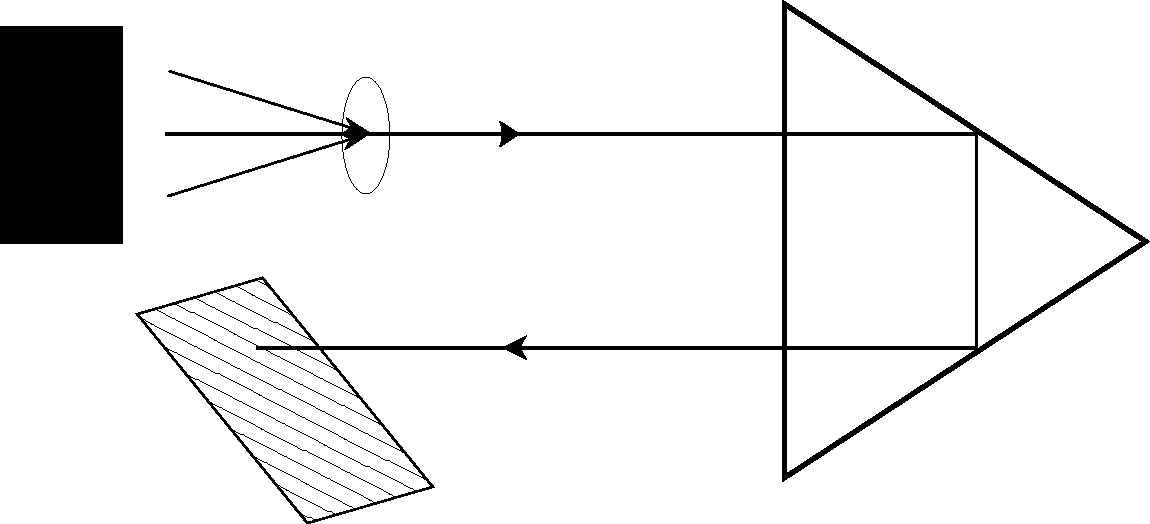
\includegraphics[height=5cm]{./linediagram.pdf}
%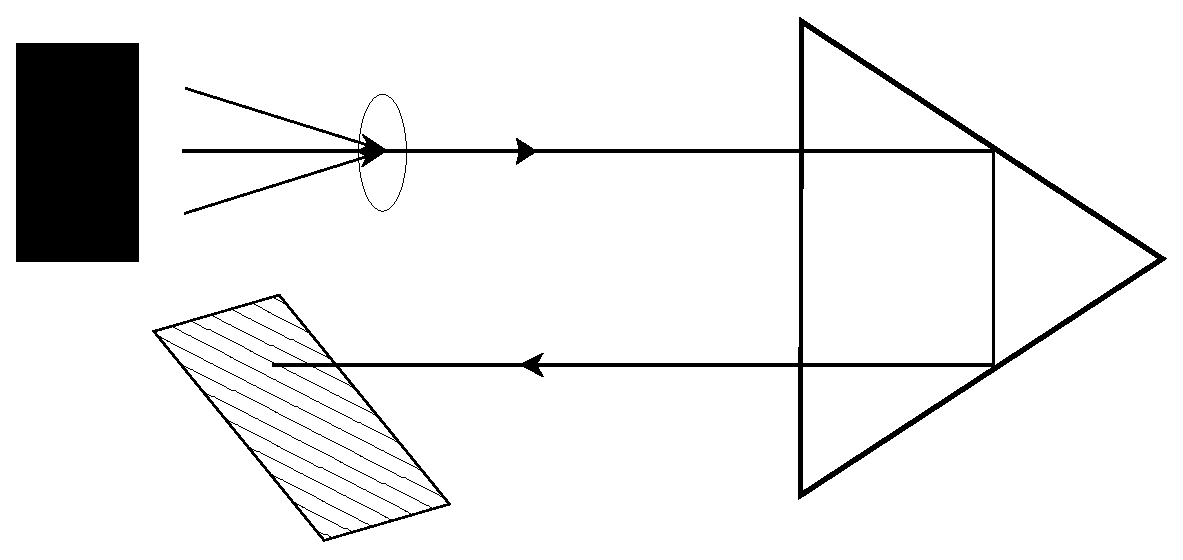
\includegraphics[height=5cm]{./linediagram.eps}
\caption{This is an example of a numbered caption. \label{kuva1}}
\end{figure}

\begin{figure}[htb]
\centering
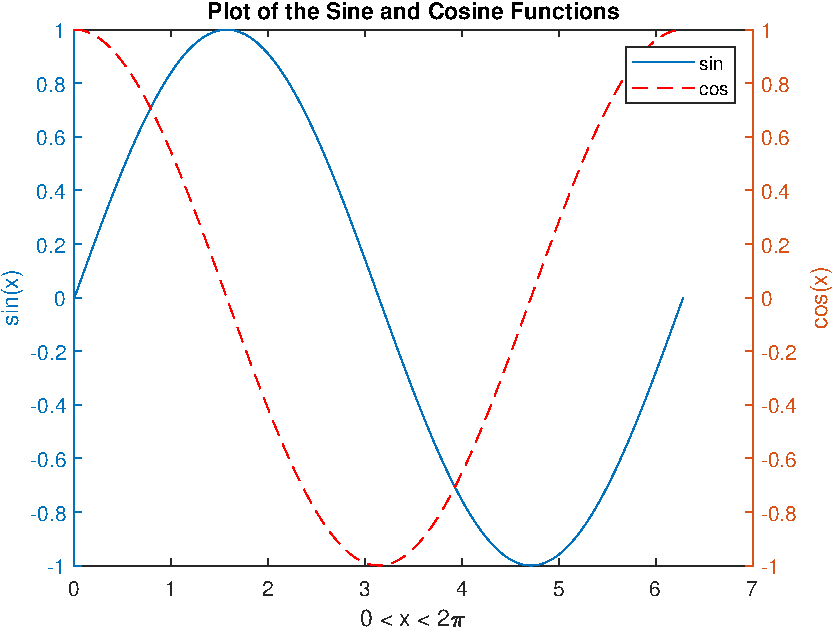
\includegraphics[height=5cm]{curves.pdf}
%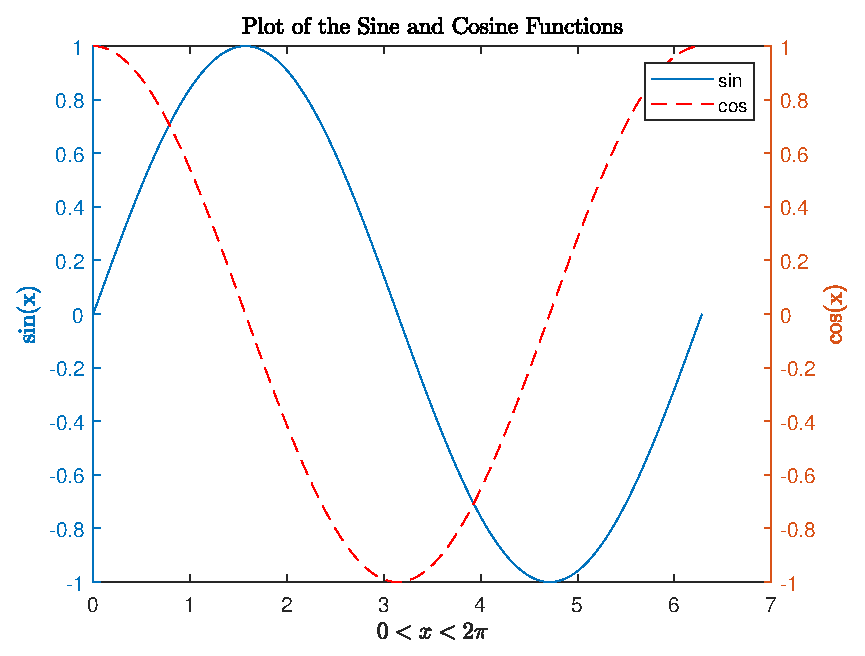
\includegraphics[height=5cm]{curves.eps}
\caption{This is an example of a MATLAB graph. \label{kuva2}}
\end{figure}


\subsection*{L\"ahdeviittausten k\"aytt\"o} 

L\"ahdeviittaukset tulee tehd\"a huolellisesti ja johdonmukaisesti
numeroviitej\"arjestelm\"an mukaisesti. Numeroviitteet j\"arjestet\"a\"an
l\"ahdeluetteloon viittausj\"arjestykseen, mutta jos l\"ahdeluettelo
on hyvin laaja (useita sivuja), j\"arjestet\"a\"an viitteet p\"a\"asanan 
mukaiseen aakkosj\"arjestykseen. Alaviitej\"arjestelm\"a\"a
\footnote{My\"osk\"a\"an alaviitteen\"a olevia kommentteja \underline{ei} suositella
k\"aytett\"aviksi.} ei k\"aytet\"a. 

Viitteen sijoittelussa noudatetaan seuraavia s\"a\"ant\"oj\"a:
Jos viite kohdistuu vain yhteen virkkeeseen tai virkkeen 
osaan, viite \cite{Kauranen} sijoitetaan virkkeen sis\"a\"an ennen virkett\"a
p\"a\"att\"av\"a\"a pistett\"a. Jos taas viite koskee tekstin useampaa
virkett\"a tai kokonaista kappaletta, sijoitetaan viite kappaleen loppuun 
pisteen j\"alkeen. \cite{Kauranen} 

\subsection*{L\"ahdeluettelo} 

L\"ahdeluettelossa esiintyy tavallisesti seuraavassa esitett\"avi\"a
l\"ahteit\"a, joista on numeroviitej\"arjestelm\"ass\"a ilmoitettava
asianomaisessa kohdassa vaaditut tiedot.

%% Esimerkki korostamisesta. Lihavoinnin sijasta on tyylikk\"a\"amp\"a\"a
%% ja luettavampaa k\"aytt\"a\"a kursiivia.
\textit{Kirjasta} ilmoitetaan seuraavat tiedot:

\begin{itemize}
\item[--]tekij\"at 
\item[--]julkaisun nimi
\item[--]painos, jos useita
\item[--]kustannuspaikka
\item[--]julkaisija tai kustantaja
\item[--]julkaisuaika
\item[--]mahdollinen sarjamerkint\"o. 
\end{itemize}

Viitteet \cite{Kauranen}--\cite{Koblitz} ovat esimerkkej\"a kirjan
esitt\"amisest\"a l\"ahdeluettelossa. Viite \cite[s.\ 83--124]{Koblitz} on
esimerkki l\"ahdeluettelossa esiintyv\"an kirjan tiettyjen sivujen
esitt\"amisest\"a tekstiss\"a.

\textit{Artikkelista} kausijulkaisussa ilmoitetaan seuraavat tiedot:

\begin{itemize}

\item[--]tekij\"at
\item[--]artikkelin nimi
\item[--]kausijulkaisun nimi
\item[--]julkaisuvuosi
\item[--]kausijulkaisun volyymi tai ilmestymisvuosi
\item[--]kausijulkaisun numero
\item[--]sivut, joilla artikkeli on.
\end{itemize}

Viitteet \cite{bcs}--\cite{Deschamps} ovat esimerkkej\"a artikkelin
esitt\"amisest\"a l\"ahdeluettelossa.

\textit{Kokoomateoksen luvusta tai osasta} ilmoitetaan seuraavat tiedot:

\begin{itemize}
\item[--]luvun tai osan tekij\"at
\item[--]luvun tai osan nimi
\item[--]maininta >>Teoksessa>>
\item[--]koko teoksen toimittajat sek\"a maininta >>(toim.)>>
\item[--]koko teoksen tai konferenssin nimi
\item[--]konferenssiesitelm\"an kyseess\"a ollessa sen pitopaikka ja -aika
\item[--]painos, jos useita
\item[--]kustannuspaikka
\item[--]julkaisija tai kustantaja, jos aihetta t\"am\"an ilmoittamiseen on
\item[--]julkaisuaika
\item[--]sivut, joilla luku tai osa on 
\item[--]mahdollinen sarjamerkint\"a.
\end{itemize}

Viitteet \cite{Sihvola}--\cite{Lindblom} ovat esimerkkej\"a
kokoomateoksen luvun tai osan esitt\"amisest\"a l\"ahdeluettelossa. 

\textit{Opinn\"aytety\"ost\"a} ilmoitetaan seuraavat tiedot:

\begin{itemize}
\item[--]tekij\"a
\item[--]ty\"on nimi
\item[--]opinn\"aytety\"on tyyppi
\item[--]oppilaitoksen nimi
\item[--]osaston, laitoksen tai ohjelman nimi
\item[--]oppilaitoksen sijaintipaikka
\item[--]vuosiluku.
\end{itemize}

Viitteet \cite{Miinusmaa}--\cite{Lonnqvist} ovat esimerkkej\"a
opinn\"aytteen esitt\"amisest\"a l\"ahdeluettelossa. 

\textit{Standardista} ilmoitetaan seuraavat tiedot:

\begin{itemize}
\item[--]standardin tunnus ja numero
\item[--]standardin nimi
\item[--]painos, mik\"ali ei ole ensimm\"ainen
\item[--]julkaisupaikka
\item[--]julkaisija
\item[--]julkaisuvuosi
\item[--]sivum\"a\"ar\"a.
\end{itemize}
Viite \cite{sfs} on esimerkki standardin esitt\"amisest\"a opinn\"aytteen
l\"ahdeluettelossa. 

\textit{Haastattelusta} ilmoitetaan seuraavat tiedot:

\begin{itemize}
\item[--]haastatellun henkil\"on nimi
\item[--]haastatellun henkil\"on arvo tai asema
\item[--]haastatellun henkil\"on edustama organisaatio
\item[--]organisaation osoite
\item[--]maininta siit\"a, ett\"a kyseess\"a on haastattelu ja haastattelun
p\"aiv\"am\"a\"ar\"a. 
\end{itemize}

Viite \cite{haastattelu} on esimerkki 
haastattelun esitt\"amisest\"a l\"ahdeluettelossa.

Osa s\"ahk\"oisess\"a muodossa olevista artikkeleista on saatavissa my\"os
painettuina. \textit{Vain verkosta saatavissa olevasta artikkelista} esitet\"a\"an
seuraavat tiedot:

\begin{itemize}
\item[--]tekij\"at
\item[--]artikkelin nimi
\item[--]kausijulkaisun nimi
\item[--]viestintyyppi
\item[--]laitos tai volyymi
\item[--]kausijulkaisun yksitt\"aist\"a osaa koskeva merkint\"a tai numero
\item[--]julkaisuvuosi tai maininta >>P\"aivitetty>> ja p\"aivitysaika
\item[--]maininta >>Viitattu>> ja viittaamisen ajankohta 
\item[--]maininta >>Saatavissa>> ja URL tai 
        maininta >>DOI>> ja DOI-numero (DOI=Digital Object Identifier).
\end{itemize}

Viitteet \cite{Ribeiro}--\cite{kone} ovat esimerkkej\"a s\"ahk\"oisess\"a
muodossa olevan artikkelin esitt\"amisest\"a opinn\"aytteen
l\"ahdeluettelossa.  Viitteet \cite{Ribeiro} ja \cite{Stieber} ovat
saatavissa sek\"a painettuna ett\"a verkosta, joten viitteiden esitystapa
mukailee painetun artikkelin viitteen esitystapaa, mutta sen lis\"aksi
kerrotaan julkaisun olevan verkkolehti ja lehden olevan saatavissa
my\"os painettuna.  Viite \cite{kone} on saatavissa vain verkosta ja
siit\"a esitet\"a\"an yll\"a vaaditut tiedot.

Valitettavasti s\"ahk\"oisess\"a muodosssa olevasta artikkelista ei ole aina 
saatavissa lai\-tos-, volyymi- tai numerotietoja.

\textit{S\"ahk\"oisess\"a muodossa olevasta opinn\"aytety\"ost\"a} ilmoitetaan
seuraavat tiedot:
 
\begin{itemize}
\item[--]tekij\"a
\item[--]ty\"on nimi
\item[--]viestintyyppi
\item[--]opinn\"aytety\"on tyyppi
\item[--]oppilaitoksen nimi
\item[--]osaston, laitoksen tai ohjelman nimi
\item[--]oppilaitoksen sijaintipaikka
\item[--]vuosiluku
\item[--]viittamisen ajankohta
\item[--]maininta >>Saatavissa>> ja URL tai 
        maininta >>DOI>> ja DOI-numero.
\end{itemize}

Viite \cite{Adida} on esimerkki s\"ahk\"oisess\"a muodossa olevan
opinn\"aytteen esitt\"amisest\"a l\"ahdeluettelossa.

Viite \cite{viittaaminen} on esimerkki itsen\"aisen kirjoituksen sis\"alt\"av\"ast\"a
verkkosivusta. T\"allainen l\"ahde on rinnastettavissa erillisteokseen.
\textit{Verkkosivusta} esitet\"a\"an tiedot:

\begin{itemize}
\item[--] tekij\"at
\item[--] otsikko
\item[--] maininta >>P\"aivitetty>> ja p\"aivitysaika 
\item[--] maininta >>Viitattu>> ja viittaamisen ajankohta
\item[--] Maininta >>Saatavissa>> ja URL.
\end{itemize}

Joskus verkkosivun kirjoitus on jaettu useammalle sivulle, jolloin
l\"ahdeluetteloon kirjataan vain sellainen verkko-osoite, joka koskee
koko kirjoitusta tai sen etusivua, ellei sitten 
todella tarkoiteta kirjoituksen yksitt\"aist\"a sivua. 

\subsection*{Muuta huomioitavaa l\"ahdeluettelossa}

%% Muutos vanhoihin ohjeisiin koskien kielt\"a.
L\"ahdeluettelossa ty\"on ja julkaisun nimi kirjoitetaan alkuper\"aisess\"a
muodossaan. Julkaisijan kotipaikka kirjoitetaan alkukielisess\"a
muodossaan.

Viittamista koskevassa suomalaisessa standardissa
SFS 5342 \cite{sfs} vaaditaan julkaisuista ilmoitettavaksi my\"os ISBN- tai
ISSN-numerot, mutta n\"aiss\"a opinn\"ayteohjeissa ei ISBN- ja 
ISSN-numeroita vaadita. 

\clearpage

\section{Research material and methods}
%\section{Tutkimusaineisto ja -menetelm\"at}

T\"ass\"a osassa kuvataan k\"aytetty tutkimusaineisto ja
tutkimuksen metodologiset valinnat, sek\"a
kerrotaan tutkimuksen toteutustapa ja k\"aytetyt menetelm\"at. 

\clearpage

\section{Results}
%\section{Tulokset}

T\"ass\"a osassa esitet\"a\"an tulokset ja vastataan tutkielman alussa
esitettyihin tutkimuskysymyksiin. Tieteellisen kirjoitelman
arvo mitataan t\"ass\"a osassa esitettyjen tulosten perusteella. 

%% Huomaa seuraavassa kappaleessa lainausmerkkien ulkopuolella piste, 
%% koska piste ei lopeta lainattua tekstinp\"atk\"a\"a.
%% Jos lainattu tekstinp\"atk\"a loppuu v\"alimerkkiin, tulee v\"alimerkki
%% lainausmerkkien sis\"alle: 
%% "Et tu, Brute?" sanoi Caesar kuollessaan.
Tutkimustuloksien merkityst\"a on aina syyt\"a arvioida ja tarkastella
kriittisesti.  Joskus tarkastelu voi olla t\"ass\"a osassa, mutta se
voidaan my\"os j\"att\"a\"a viimeiseen osaan, jolloin viimeisen osan nimeksi
tulee >>Tarkastelu>>. Tutkimustulosten merkityst\"a voi arvioida my\"os
>>Johtop\"a\"at\"okset>>-otsikon alla viimeisess\"a osassa. 

T\"ass\"a osassa on syyt\"a my\"os arvioida tutkimustulosten luotettavuutta.
Jos tutkimustulosten merkityst\"a arvioidaan >>Tarkastelu>>-osassa,
voi luotettavuuden arviointi olla my\"os siell\"a. 

\clearpage

\section{Summary} 
%\section{Yhteenveto}

Opinn\"aytteen tekij\"a vastaa siit\"a, ett\"a opinn\"ayte on t\"ass\"a dokumentissa
ja opinn\"aytteen tekemist\"a k\"asittelevill\"a luennoilla sek\"a
harjoituksissa annettujen ohjeiden mukainen muotoseikoiltaan,
rakenteeltaan ja ulkoasultaan.



\clearpage
%% L\"ahdeluettelo

\thesisbibliography

\begin{thebibliography}{99}

%% Alla pilkun j\"alkeen on pakotettu oikea v\"ali \<v\"alily\"onti>-merkeill\"a.
\bibitem{Kauranen} Kauranen,\ I., Mustakallio,\ M. ja Palmgren,\ V.
  \textit{Tutkimusraportin kirjoittamisen opas opinn\"aytety\"on
    tekij\"oille.}  Espoo, Teknillinen korkeakoulu, 2006.

\bibitem{Itkonen} Itkonen,\ M. \textit{Typografian k\"asikirja.} 3.\
  painos.  Helsinki, RPS-yhti\"ot, 2007.

\bibitem{Koblitz} Koblitz,\ N. \textit{A Course in Number Theory and
    Cryptography. Graduate Texts in Mathematics 114.}  2.\ painos. New
  York, Springer, 1994.

%% Kun on useampi nimikirjain, jokaisen nimikirjaimen v\"aliin
%% kuuluu v\"alily\"onti. Oikea v\"alin m\"a\"ar\"a on saatu \<v\"alily\"onnill\"a>
\bibitem{bcs} Bardeen,\ J., Cooper,\ L.\ N. ja Schrieffer,\ J.\ R.
  Theory of Superconductivity. \textit{Physical Review,} 1957, vol.\
  108, nro~5, s.\ 1175--1204.

\bibitem{Deschamps} Deschamps,\ G.\ A. Electromagnetics and
  Differential Forms. \textit{Proceedings of the IEEE,} 1981, vol.\
  69, nro~6, s.\ 676--696.

%% Alla esimerkki englanninkielisen tavuttamisen pakottamisesta.
%% Oletusarvoisesti k\"aytet\"a\"an suomalaista tavutusta, mutta viitteiss\"a
%% esiintyy usein muunkielisi\"a lauseita, jotka tulevat siten tavutetuksi
%% suomen kielen s\"a\"ant\"ojen mukaan. T\"am\"an voi korjata \foreignlanguage-
%% komennolla, jonka ensimm\"ainen parametri on vieraan kielen nimi ja toinen 
%% on vieraalla kielell\"a tavutettava teksti. 
\bibitem{Sihvola} Sihvola,\ A.\ et al.
  \foreignlanguage{english}{Interpretation of measurements of helix 
    and bihelix superchiral structures.}
  Teoksessa: Jacob,\ A.\ F. ja
  Reinert,\ J. (toim.) \textit{Bianisotropics '98 7th International
    Conference on Complex Media.}  Braunschweig, 3.--6.6.1998.
  Braunscweig, Technische Universit\"at Braunschweig, 1998, s.\
  317--320.

%% Alla on suomalainen yhdistelm\"asukunimi. Sen nimien v\"aliss\"a 
%% k\"aytet\"a\"an yhdysmerkki\"a l. tavuviivaa, kirjoitetaan -.
\bibitem{Lindblom} Lindblom-Yl\"anne,\ S. ja Wager,\ M.  Tieteellisten
  opinn\"aytet\"oiden ohjaaminen. Teoksessa: Lindblom-Yl\"anne,\ S. ja
  Nevgi,\ A. (toim.) \textit{Yliopisto- ja korkeakouluopettajan
    k\"asikirja.}  Helsinki, WSOY, 2004, s.\ 314--325.
 
\bibitem{Miinusmaa} Miinusmaa,\ H. Neliskulmaisen rei\"an poraamisesta
  kolmikulmaisella poralla. Diplomity\"o, Teknillinen korkeakoulu,
  konetekniikan osasto, Espoo, 1977.

%% T\"ass\"a taas pakotettu englanninkielinen tavutus. 
%% Pedanttinen kirjoittaja pakottaa tietysti jokaiseen englanninkieliseen
%% lauseeseen englannin tavutuksen, mutta t\"ass\"a esityksess\"a ei n\"ain ole
%% tehty selvyyden ja l\"ahdekoodin luettavuuden takia. 
\bibitem{Loh} Loh,\ N.\ C. High-Resolution Micromachined
  Interferometric Accelerometer. Master's Thesis, Massachusetts
  Institute of Technology, Cambridge,
  \foreignlanguage{english}{Massachusetts,} 1992.

\bibitem{Lonnqvist} L\"onnqvist,\ A.
  \foreignlanguage{english}{Applications of hologram-based compact
    range: antenna radiation pattern, radar cross section, and
    absorber reflectivity measurements.}
  V\"ait\"oskirja, Teknillinen korkeakoulu, s\"ahk\"o- ja tietoliikennetekniikan
  osasto, 2006.

\bibitem{sfs} SFS 5342. Kirjallisuusviitteiden laatiminen. 2.\ painos.
  Helsinki, Suomen standardisoimisliitto, 2004. 20~s.

\bibitem{haastattelu} Palmgren,\ V. Suunnittelija. Teknillinen
  korkeakoulu, kirjasto. Otaniementie 9, 02150 Espoo. Haastattelu
  15.1.2007.

\bibitem{Ribeiro} Ribeiro,\ C.\ B., Ollila,\ E. ja Koivunen,\ V.
  \foreignlanguage{english}{Stochastic Maximum-Likelihood Method for
    MIMO Propagation Parameter Estimation.}
 \textit{IEEE Transactions
    on Signal Processing,} verkkolehti, vol.\ 55, nro~1, s.\ 46--55.
  Viitattu 19.1.2007. Lehti ilmestyy my\"os painettuna. DOI:
  10.1109/TSP.2006.882057.

\bibitem{Stieber} Stieber,\ T. GnuPG Hacks. \textit{Linux Journal,}
  verkkolehti, 2006, maaliskuu, nro~143. Viitattu 19.1.2007. Lehti
  ilmestyy my\"os painettuna. Saatavissa:
  \url{http://www.linuxjournal.com/article/8732.}

\bibitem{kone} Pohjois-Koivisto,\ T. Voiko kone tulevaisuudessa arvata
  tahtosi?  \textit{Apropos,} verkkolehti, helmikuu, nro~1, 2005.
  Viitattu 19.1.2007.  Saatavissa:
  \url{http://www.apropos.fi/1-2005/prima.php.}

\bibitem{Adida} Adida,\ B.  Advances in Cryptographic Voting Systems.
  Verkkodokumentti. Ph.D.\ Thesis, Massachusetts Institute of
  Technology, Cambridge, 
  \foreignlanguage{english}{Massachusetts,}
  2006. Viitattu 19.1.2007.  Saatavissa:
  \url{http://crypto.csail.mit.edu/~cis/theses/adida-phd.pdf.}

\bibitem{viittaaminen} Kilpel\"ainen,\ P. WWW-l\"ahteisiin viittaaminen
  tutkielmatekstiss\"a. Verkkodokumentti. P\"aivitetty 26.11.2001.
  Viitattu 19.1.2007. Saatavissa:
  \url{http://www.cs.uku.fi/~kilpelai/wwwlahteet.html.}

\end{thebibliography}

%% Appendices
%% If you don't have appendices, remove \clearpage and \thesisappendix below.
\clearpage

\thesisappendix

\section{Esimerkki liitteest\"a\label{LiiteA}}

Liitteet eiv\"at ole opinn\"aytteen kannalta v\"altt\"am\"att\"omi\"a ja 
opinn\"aytteen tekij\"an on 
kirjoittamaan ryhtyess\"a\"an hyv\"a ajatella p\"arj\"a\"av\"ans\"a ilman liitteit\"a.
Kokemattomat kirjoittajat, jotka ovat huolissaan
tekstiosan pituudesta, paisuttavat turhan 
helposti liitteit\"a pit\"a\"akseen tekstiosan pituuden annetuissa rajoissa.
T\"all\"a tavalla ei synny hyv\"a\"a opinn\"aytett\"a.   

Liite on itsen\"ainen kokonaisuus, vaikka se t\"aydent\"a\"akin tekstiosaa.
Liite ei siten ole pelkk\"a listaus, kuva tai taulukko, vaan 
liitteess\"a selitet\"a\"an aina sis\"all\"on laatu ja tarkoitus. 

Liitteeseen voi laittaa esimerkiksi listauksia. Alla on 
listausesimerkki t\"am\"an liitteen luomisesta. 

%% Verbatim-ymp\"arist\"o ei muotoile tai tavuta teksti\"a. Fontti on monospace.
%% Verbatim-ymp\"arist\"on sis\"all\"a annettuja komentoja ei LaTeX k\"asittele. 
%% Vasta \end{verbatim}-komennon j\"alkeen jatketaan k\"asittely\"a.
\begin{verbatim}
	\clearpage
	\appendix
	\addcontentsline{toc}{section}{Liite A}
	\section*{Liite A}
	...
	\thispagestyle{empty}
	...
	teksti\"a
	...
	\clearpage
\end{verbatim}

Kaavojen numerointi muodostaa liitteiss\"a oman kokonaisuutensa:
\begin{align}
d \wedge A &= F, \label{liitekaava1}\\
d \wedge F &= 0. \label{liitekaava2}
\end{align}


\clearpage
\section{Toinen esimerkki liitteest\"a\label{LiiteB}}

%% Liitteiden kaavat, taulukot ja kuvat numeroidaan omana kokonaisuutenaan
%%
%% Equations, tables and figures have their own numbering in Appendices
%\renewcommand{\theequation}{B\arabic{equation}}
%\setcounter{equation}{0}  
%\renewcommand{\thefigure}{B\arabic{figure}}
%\setcounter{figure}{0}
%\renewcommand{\thetable}{B\arabic{table}}
%\setcounter{table}{0}

Liitteiss\"a voi my\"os olla kuvia, jotka
eiv\"at sovi leip\"atekstin joukkoon:
%% Ymp\"arist\"on figure parametrit htb pakottavat
%% kuvan t\"ah\"an, eik\"a LaTeX yrit\"a siirrell\"a niit\"a
%% hyv\"aksi katsomaansa paikkaan. 
%% Ymp\"arist\"o\"a center voi k\"aytt\"a\"a \centering-
%% komennon sijaan
%%
%% Example of a figure, note the use of htb parameters which force
%% the figure to be inserted here
\begin{figure}[htb]
\begin{center}
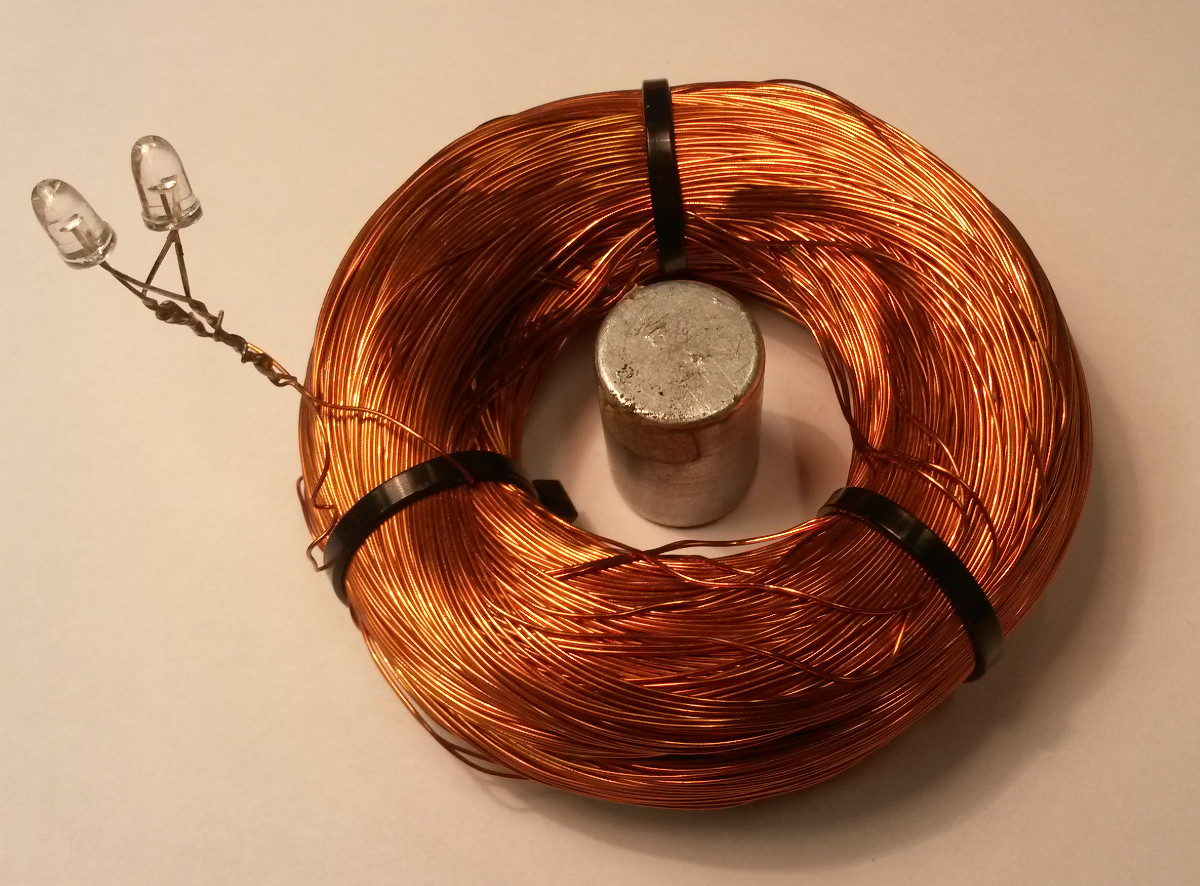
\includegraphics[height=8cm]{./ledspole.jpg}
\end{center}
\caption{Kuvateksti, jossa on liitteen numerointi}
\label{liitekuva}
\end{figure}
%%
Liitteiden taulukoiden numerointi on kuvien ja kaavojen kaltainen:
\begin{table}[htb]
\caption{Taulukon kuvateksti.}
\label{liitetaulukko}
\begin{center}
\fbox{
\begin{tabular}{lp{0.5\linewidth}}
9.00--9.55  & K\"aytett\"avyystestauksen tiedotustilaisuus (osanottajat
ovat saaneet s\"ahk\"opostitse valmistautumisteht\"av\"at, joten tiedotustilaisuus
voidaan pit\"a\"a lyhyen\"a).\\
9.55--10.00 & Testausalueelle siirtyminen
\end{tabular}}
\end{center}
\end{table}
Kaavojen numerointi muodostaa liitteiss\"a oman kokonaisuutensa:
\begin{align}
T_{ik} &= -p g_{ik} + w u_i u_k + \tau_{ik},  \label{liitekaava3} \\
n_i    &= n u_i + v_i.                      \label{liitekaava4}
\end{align}

\end{document}
